% !Mode:: "TeX:UTF-8" 



\BiSection{2.14}{Figures}

\fancyhead[R]{本题2.14由QC.Z完成}



解:

\scalebox{3}{(1)}

$I_D=I_0e^{\frac{V_{GS}}{\xi V_T}}$\textcolor{blue}{(P23的2.33)}

$g_m=\frac{\partial I_D}{\partial V_{GS}}=I_0e^{\frac{V_{GS}}{\xi V_T}}\frac{1}{\xi V_T}=\frac{I_D}{\xi V_T}$


\begin{figure}[H] %H为当前位置,!htb为忽略美学标准,htbp为浮动图形
	\begin{minipage}{\linewidth}
		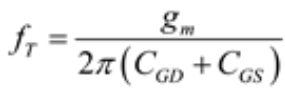
\includegraphics{2.14-1}
	\end{minipage}
\end{figure}


\begin{figure}[H] %H为当前位置,!htb为忽略美学标准,htbp为浮动图形
	\begin{minipage}{\linewidth}
		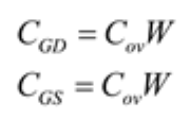
\includegraphics{2.14-2}
	\end{minipage}
\end{figure}


\begin{figure}[H] %H为当前位置,!htb为忽略美学标准,htbp为浮动图形
	\begin{minipage}{\linewidth}
		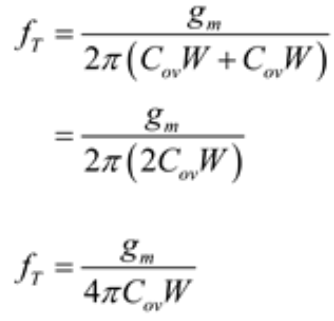
\includegraphics{2.14-3}
	\end{minipage}
\end{figure}


\begin{figure}[H] %H为当前位置,!htb为忽略美学标准,htbp为浮动图形
	\begin{minipage}{\linewidth}
		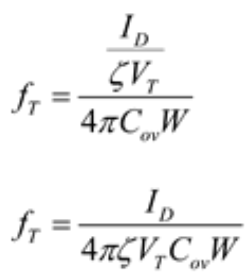
\includegraphics{2.14-4}
	\end{minipage}
\end{figure}

\scalebox{3}{(2)}

把每单位宽度重叠电容$C_{ov}\cong L_DC_{ox}$带入前式有

\begin{figure}[H] %H为当前位置,!htb为忽略美学标准,htbp为浮动图形
	\begin{minipage}{\linewidth}
		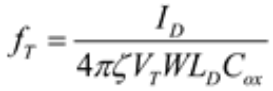
\includegraphics{2.14-5}
	\end{minipage}
\end{figure}

上一题2.13用面积律特性的特征频率表达式为

\begin{figure}[H] %H为当前位置,!htb为忽略美学标准,htbp为浮动图形
	\begin{minipage}{\linewidth}
		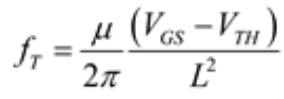
\includegraphics{2.14-6}
	\end{minipage}
\end{figure}

联立以上二式

\begin{figure}[H] %H为当前位置,!htb为忽略美学标准,htbp为浮动图形
	\begin{minipage}{\linewidth}
		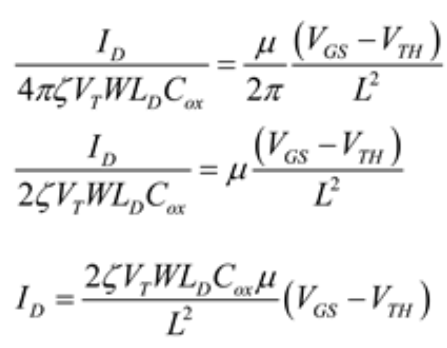
\includegraphics{2.14-7}
	\end{minipage}
\end{figure}



上式$I_D$与W成正比